\documentclass[handout]{beamer}
\usepackage[utf8]{inputenc}
\usepackage[T2A]{fontenc}
\usepackage[english]{babel}
\usepackage{graphicx}
\usepackage{array}
\usetheme{Warsaw}
\usecolortheme{wolverine}

\usepackage{fontawesome5}
\usepackage{changepage}
\usepackage{soul}
\usepackage[table]{xcolor}

\definecolor{ukraine-blue}{rgb}{0,0.34,0.72}
\definecolor{ukraine-yellow}{rgb}{1,0.84,0}

\setbeamercolor{title}{fg=ukraine-blue,bg=ukraine-yellow}
\setbeamercolor{frametitle}{fg=ukraine-blue,bg=ukraine-yellow}
\setbeamercolor{section in head/foot}{fg=ukraine-blue}
\setbeamercolor{title in head/foot}{fg=ukraine-blue,bg=ukraine-yellow}
\setbeamercolor{author in head/foot}{fg=ukraine-yellow,bg=ukraine-blue}

\definecolor{darkblue}{rgb}{0,0,0.8}
\definecolor{darkgreen}{rgb}{0,0.6,0}
\definecolor{darkred}{rgb}{1,0,0}

\title[CLC 2021--2024]{{CLC activities 2021--2024:} \\ a personal memoir}
\author[Andrew Lelechenko]{Andrew Lelechenko \\ \texttt{andrew.lelechenko@gmail.com}}
\date{MuniHac, 12.10.2024}

\begin{document}

\begin{frame}
  \titlepage

\end{frame}

\begin{frame}{What is CLC?}

\begin{columns}[T]
  \begin{column}{.45\textwidth}

\bigskip\bigskip

\begin{itemize}[<+->]
\item CLC stands for Core Libraries Committee.

\bigskip\bigskip

\item Core Libraries are libraries governed by CLC.

\bigskip\bigskip

\item {\tt let x = x in x}
\end{itemize}

\end{column}

\begin{column}{.55\textwidth}
  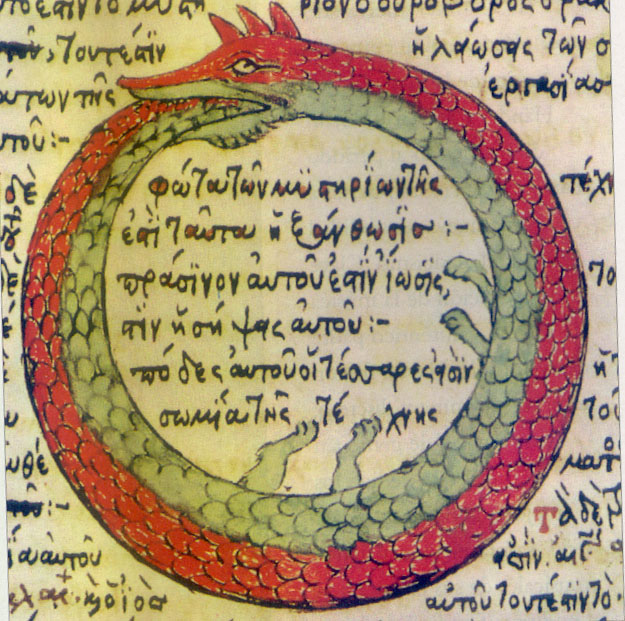
\includegraphics[width=\textwidth]{uroboros.jpg}
\end{column}

\end{columns}

\end{frame}

\begin{frame}{Quiz time}

\begin{itemize}

\def\yes{\textcolor{darkgreen}{Yes.}}
\def\no{\textcolor{darkred}{No.}}

\item CLC appoints Hackage trustees. \no
\item CLC maintains {\tt bytestring} package. \no
\item CLC approves changes to {\tt Data.Text}. \no
\item You need CLC assent to add new GHC RTS flags. \yes
\item CLC can amend Haskell Package Versioning Policy. \yes
\item CLC owns {\tt haskeline} and {\tt terminfo} packages. \yes
\item Bug fixes in {\tt base} do not need CLC assent. \yes
\item Changes to {\tt ghc-internal} are out of scope for CLC. \no
\item Moving implementation of {\tt base} elsewhere involves CLC. \no
\item CLC is responsible for stability of {\tt base}. \no
% CLC is politically neutral.
\item Adding class laws for {\tt Num} falls under CLC purview. \yes
\item Documentation for {\tt Data.List} must be verified by CLC. \no

\end{itemize}

\end{frame}

\begin{frame}{CLC purview}

\begin{columns}[T]
  \begin{column}{.47\textwidth}

\begin{itemize}[<+->]
\bigskip
\item User-visible changes to API of {\tt base} package.
\bigskip
\item Governance of designated so called ``Core'' packages.
\bigskip
\item Haskell Package Versioning Policy aka PVP.
\end{itemize}

\end{column}

\begin{column}{.53\textwidth}
  
\includegraphics[width=\textwidth]{triskelion.png}
\end{column}

\end{columns}

\end{frame}

\begin{frame}{PVP: Haskell Package Versioning Policy}

\begin{itemize}[<+->]

\item PVP 1.0 lives at {\tt https://pvp.haskell.org}
\item PVP 1.1 is work in progress since 2019.
\item PVP contains normative and non-normative sections.
\item Non-normative changes (FAQ, decision tree, etc.) can be made by CLC alone.
\item The definition of breaking changes and versioning schema require also Hackage admins to agree.

\end{itemize}

\medskip

\centerline{
\includegraphics[width=0.58\textwidth]{pvp.jpg}}

\end{frame}

\begin{frame}{Boot and core packages --- 1}

% * Which packages are prime candidates for adoption?
% * Why usual Hackage takeover process is insufficient?
% * Why maintainers abandon packages and lose engagement?

\vspace{-0.5em}

\begin{table}[c]
\begin{tabular}{lccc}
Package          & Boot              & Core 2021 & Core 2024          \\
\hline
array            & +                 & +         & +                  \\
binary           & +                 &           & \cellcolor{green}+ \\
bytestring       & +                 & +         & +                  \\
Cabal            & +                 &           & \cellcolor{green}+ \\
Cabal-syntax     & +                 &           & \cellcolor{green}+ \\
cabal-install    &                   &           & \cellcolor{green}+ \\
cabal-install-solver &               &           & \cellcolor{green}+ \\
containers       & \cellcolor{red}+  &           &                    \\
deepseq          & +                 & +         & +                  \\
directory        & +                 & +         & +                  \\
entropy          &                   &           & \cellcolor{green}+ \\
exceptions       & \cellcolor{red}+  &           &                    \\
file-io          & +                 &           & \cellcolor{green}+ \\
filepath         & +                 & +         & +                  \\
haskeline        & +                 &           & \cellcolor{green}+ \\
hpc              & +                 &           & \cellcolor{green}+ \\
mtl              & +                 & +         & +                  \\
\end{tabular}
\end{table}

\end{frame}

\begin{frame}{Boot and core packages --- 2}

\begin{table}[c]
\begin{tabular}{lccc}
Package          & Boot              & Core 2021 & Core 2024          \\
\hline
os-string        & +                 &           & \cellcolor{green}+ \\
parsec           & \cellcolor{red}+  &           &                    \\
pretty           & \cellcolor{red}+  &           &                    \\
primitive        &                   & +         & +                  \\
process          & +                 & +         & +                  \\
random           &                   & +         & +                  \\
stm              & +                 & +         & +                  \\
template-haskell & +                 & +         & +                  \\
terminfo         & +                 &           & \cellcolor{green}+ \\
text             & +                 & +         & +                  \\
time             & \cellcolor{red}+  &           &                    \\
transformers     & +                 &           & \cellcolor{green}+ \\
unix             & +                 & +         & +                  \\
vector           &                   & +         & +                  \\
Win32            & +                 & +         & +                  \\
xhtml            & +                 &           & \cellcolor{green}+ \\
\end{tabular}
\end{table}

\end{frame}

\begin{frame}{CLC proposals --- 1}

\begin{itemize}[<+->]
\item By summer 2021 CLC was in crisis, down to 2 active members.
\item In August CLC was rebooted with a goal to provide for better engagement
of committee members.
\item In September a fresh batch of CLC members was elected.
\bigskip
\item To be able to get things done, \\
      we got a new home for proposals at GitHub instead of mail.
\item To manage community expectations, \\
      we developed a lightweight, but precise proposal process.
\item To prevent burning out, \\
      we brought our remit in line with our capabilities.
\bigskip
\item CLC proposal process is asynchronous, transparent and written communication.
\end{itemize}

\end{frame}

\begin{frame}{CLC proposals --- 2}

\begin{itemize}[<+->]

\def\tt{}

\item Total number of CLC proposals: {\bf 249}
\item Rate of proposals: {\bf 7} per month
\item Approved proposals: {\bf 125}
\item Declined proposals: {\bf 9}

% Declining is bad for morale.
% The role of a chair is for every proposal to succeed.
% Every proposer deserves at least one ally, the chair is meant to provide such support.

% GHC Proposals: Total number of GHC proposals: 440
% GHC Proposals: Rate of proposals:  5 per month
% GHC Proposals: Approved proposals: 149
% GHC Proposals: Need revision:      30
% GHC Proposals: Declined proposals: 16

\medskip

\item Median  time from creation to decision: {\bf 39} days
\item Average time from creation to decision: {\bf 80} days
\item Median  time from creation to approval: {\bf 50} days
\item Average time from creation to approval: {\bf 81} days

% GHC Proposals: Median  time from creation to decision: 101 days
% GHC Proposals: Average time from creation to decision: 181 days
% GHC Proposals: Median  time from creation to approval: 100 days
% GHC Proposals: Average time from creation to approval: 165 days

\medskip

\item The fastest approval:
  {\bf 2} hours \\ {\small for {\it Use {\tt HasCallStack} and {\tt error} in {\tt GHC.List} and {\tt .NonEmpty}}}
\item $2^{nd}$ fastest approval:
  {\bf 34} hours \\ {\small for {\it Remove default method from {\tt Bitraversable}}}
\item $2^{nd}$ slowest approval:
  {\bf 375} days \\ {\small for {\it Exception backtrace proposal: Part 4: Rethrowing}}
\item The slowest approval:
  {\bf 395} days \\ {\small for {\it {\tt base} changes for exception backtrace proposal}}

% GHC Proposals: Fastest approval:
%   8 days for "Adjust warning category syntax"
% GHC Proposals: 2nd fastest approval:
%   11 days for "Remove dot from characters allowed in overloaded labels"
% GHC Proposals: 2nd slowest approval:
%   980 days for "Fine-grained unused warnings"
% GHC Proposals: Slowest approval:
%   1112 days for "Decorate exceptions with backtrace information"

\end{itemize}
\end{frame}

\begin{frame}{CLC proposals --- 3}
\begin{itemize}[<+->]

\def\tt{}

\item Total activity: {\bf 6302} comments
\item Median  activity per proposal:          {\bf 17} comments
\item Average activity per proposal:          {\bf 25} comments
\item Median  activity per approved proposal: {\bf 21} comments
\item Average activity per approved proposal: {\bf 30} comments
\item The least active approved proposal:
   {\bf 1} comment \\ for {\it Export {\tt List} from {\tt GHC.List}}
\item $2^{nd}$ least active approved proposal:
   {\bf 6} comments \\ for {\it Make casts between words and floats real primops}
\item $2^{nd}$ most active:
   {\bf 171} comments \\ for {\it Remove method {\tt (/=)} from class {\tt Eq}}
\item The most active:
   {\bf 177} comments \\ for {\it Add warning to {\tt Data.List.\{head,tail\}}}

% The very first proposal remains unimplemented!

% There is a certain threshold of technical competence,
% which no process can ameliorate.

% GHC Proposals: Total activity: 15975 comments
% GHC Proposals: Median  activity per proposal:          23 comments
% GHC Proposals: Average activity per proposal:          36 comments
% GHC Proposals: Median  activity per approved proposal: 31 comments
% GHC Proposals: Average activity per approved proposal: 51 comments
% GHC Proposals: 2nd most active:
%   313 comments for "Lambda expressions with guards and multiple clauses (was: `\ of`, -XMultiWayLambda)"
% GHC Proposals: Most active:
%   519 comments for "RecordDotSyntax language extension proposal"

\end{itemize}
\end{frame}

\begin{frame}{CLC proposals --- 4}

\def\tt{}

\begin{table}[c]
\begin{tabular}{lrr}
Release & Date & Count\\ \hline
base-4.16 & 28 Feb 2022 & {\bf 1} \\
base-4.17 &  7 Aug 2022 & {\bf 11} \\
base-4.18 & 11 Mar 2023 & {\bf 24} \\
base-4.19 &  9 Oct 2023 & {\bf 25} \\
base-4.20 & 14 May 2024 & {\bf 33} \\
base-4.21 & TBA & {\bf 21} \\
\end{tabular}
\end{table}

\medskip\pause

\begin{itemize}[<+->]
\item Open proposals: {\bf 13}
\item Median  age for open proposals: {\bf 6} days
\item Average age for open proposals: {\bf 63} days
\item The newest open proposal:
   {\bf 1} day \\ {\small for {\it Formally deprecate modules informally marked unstable in \#146}}
\item The oldest open proposal:
  {\bf 691} days \\ {\small for {\it Make NonEmpty functions less gratuitously lazy}}

% Strict no-show rejection policy.

% GHC Proposals: Open proposals: 116
% GHC Proposals: Median  age for open proposals: 1127 days
% GHC Proposals: Average age for open proposals: 1209 days
% GHC Proposals: Newest open proposal:
%   11 days for "Amend Import Shadowing proposal to match Haskell 2010 section 5.2.5"
% GHC Proposals: Oldest open proposal:
%   2943 days for "Mutable constructor fields"

\end{itemize}
\end{frame}

\begin{frame}{How to get your proposal approved?}
\begin{itemize}[<+->]

\item Be patient.
\item Be persistent.
\item Be clear.
\item Be precise.
\item Stand on the shoulders of giants: find prior art.
\item Think hard about possible breakage and its mitigation.
\item Follow the \st{white rabbit} proposal process.

\end{itemize}
\end{frame}

\begin{frame}{CLC Election January 2025}

\begin{columns}[T]
  \begin{column}{.61\textwidth}

\begin{itemize}[<+->]
\item Bandwidth to analyse and contribute opinions for 6--8 proposals per month.
\item Communication and governing-the-commons skills.
\item Determination to see proposals through to their timely completion.
\item We are not looking for the biggest galaxy brain in the room.
\item We hope to build a broad sample of the community.
\end{itemize}

\end{column}

\begin{column}{.39\textwidth}
  \bigskip\medskip
  
\includegraphics[width=\textwidth]{galaxy-brain.jpg}
\end{column}

\end{columns}

% Discuss issues with self-selection process and degrading diversity.

\end{frame}

\begin{frame}{How you can help CLC}

\begin{columns}[T]
  \begin{column}{.53\textwidth}

\begin{itemize}[<+->]

\item Be welcome to participate in~CLC~discussions.
\bigskip

\item Pick up an abandoned proposal and~work towards completion.
\bigskip

\item Volunteer to write CLC blog at~Haskell.org.
\bigskip

\item Raise more new proposals.
\bigskip

\item Like and subscribe to {\tt github.com/haskell/core-libraries-committee}.

% Committees live and die on community engagement.
% Community gives us purpose.

\end{itemize}

\end{column}

\begin{column}{.47\textwidth}
  
\includegraphics[width=\textwidth]{wants-you.jpg}
\end{column}

\end{columns}

\bigskip\pause

\centerline{\Huge Thanks all!}

\end{frame}

\end{document}
